% Solution: Tadelis (2013) Exercise 7.6 "Entering an Industry". Input by \solitem.
% New in the 50-item list. Check: check_D.py.
\begin{exsol}{Tadelis Exercise 7.6}{148--149}{Foundations}{1}
\asked (a) A game tree with payoffs that represent the stated rankings; (b) the number of pure
strategies of each player; (c) all Nash equilibria.

\method Extensive form and game trees (Tadelis \S7.1, pp.~130--137); pure strategies as complete
plans (\S7.2.1, p.~137); the normal-form representation of a game tree (\S7.2.3, p.~143); Nash
equilibrium and paths of play, on and off the equilibrium path (\S7.3 and Def.~7.8, pp.~145--146).
The question stops at Nash equilibrium; which equilibrium survives sequential rationality is
Tadelis \S8.1 (Def.~8.1, p.~152) and Lecture~4, slides~13 and~17 (the entry-deterrence logic of
the Brexit case, slides~9--11).

\solution
\textbf{(a) Tree.} Ordinal payoffs suffice, since only the rankings are given. Write $\mathit{In}$
and $\mathit{Out}$ for player~1's choice and $A$ (accommodate), $F$ (fight) for player~2's. The
rankings are
\[
  \text{player 1: } (\mathit{In},A) \succ \mathit{Out} \succ (\mathit{In},F), \qquad
  \text{player 2: } \mathit{Out} \succ (\mathit{In},A) \succ (\mathit{In},F).
\]
Player~1's middle outcome must be $\mathit{Out}$ and player~2's must be $(\mathit{In},A)$, the only
outcomes not named as best or worst. Payoffs $2,1,0$ in that order give
\begin{center}
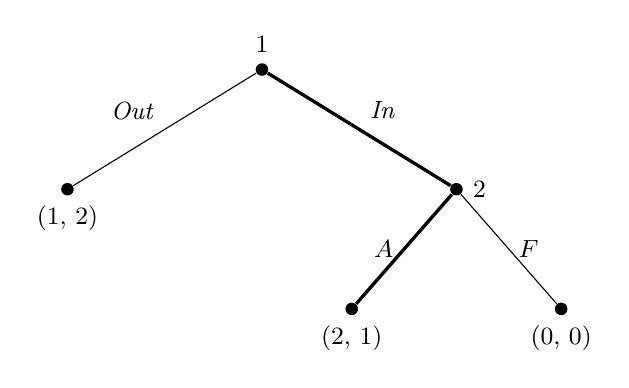
\begin{tikzpicture}[scale=0.95,dot/.style={circle,fill,inner sep=1.6pt},
  every node/.style={font=\small}]
  \node[dot,label=above:{1}] (r) at (0,0) {};
  \node[dot,label=below:{$(1,\,2)$}] (o) at (-2.6,-1.6) {};
  \node[dot,label=right:{2}] (i) at (2.6,-1.6) {};
  \node[dot,label=below:{$(2,\,1)$}] (a) at (1.2,-3.2) {};
  \node[dot,label=below:{$(0,\,0)$}] (f) at (4.0,-3.2) {};
  \draw (r) -- node[above left] {$\mathit{Out}$} (o);
  \draw[very thick] (r) -- node[above right] {$\mathit{In}$} (i);
  \draw[very thick] (i) -- node[left] {$A$} (a);
  \draw (i) -- node[right] {$F$} (f);
\end{tikzpicture}\\[2pt]
{\footnotesize Payoffs $(u_1,u_2)$; thick branches = backward-induction choices (used below).}
\end{center}
Any numbers with the same rankings give the same answers to (b) and (c).

\textbf{(b) Pure strategies.} Each player has one information set with two actions, so
$S_1 = \{\mathit{In},\mathit{Out}\}$ and $S_2 = \{A,F\}$: two pure strategies each. Player~2's
strategy is a plan for the node after entry, and it is part of the profile even when player~1
stays out.

\textbf{(c) Nash equilibria.} The normal form, with best replies underlined:
\begin{center}
\begin{tabular}{r|c|c|}
\multicolumn{1}{r}{} & \multicolumn{1}{c}{$A$} & \multicolumn{1}{c}{$F$}\\ \cline{2-3}
$\mathit{In}$  & $\br{2},\ \br{1}$ & $0,\ 0$ \\ \cline{2-3}
$\mathit{Out}$ & $1,\ \br{2}$ & $\br{1},\ \br{2}$ \\ \cline{2-3}
\end{tabular}
\end{center}
\emph{Pure.} $(\mathit{In},A)$ and $(\mathit{Out},F)$. Against $A$, $\mathit{In}$ gives $2 > 1$;
against $F$, $\mathit{Out}$ gives $1 > 0$. Against $\mathit{In}$, $A$ gives $1 > 0$; against
$\mathit{Out}$, player~2 gets 2 with either action, so $F$ is a (weak) best reply.

\emph{Mixed.} Let $p = \Pr(\mathit{In})$ and $f = \Pr(F)$.
\begin{itemize}
  \item If $p > 0$, then $u_2(A) - u_2(F) = p\cdot(1 - 0) > 0$, so $f = 0$, and then $\mathit{In}$
  is player~1's unique best reply ($2 > 1$): $p = 1$. This is $(\mathit{In},A)$.
  \item If $p = 0$, player~2 is indifferent, so any $f$ is a best reply. $\mathit{Out}$ is a best
  reply for player~1 iff
  \[
    u_1(\mathit{Out}) = 1 \;\ge\; u_1(\mathit{In}) = 2(1-f) + 0\cdot f
    \iff f \ge \tfrac12 .
  \]
\end{itemize}
So the set of all Nash equilibria is
\[
  \{(\mathit{In},A)\} \;\cup\; \bigl\{(\mathit{Out},\ \sigma_2) : \sigma_2(F) \ge \tfrac12\bigr\},
\]
a single entry equilibrium plus a continuum of deterrence equilibria, $(\mathit{Out},F)$ among them.

\textbf{Which are sequentially rational.} At player~2's node, $A$ gives $1 > 0$. Every equilibrium
of the second family puts weight $f \ge \frac12$ on $F$ at a node that is off the equilibrium path
(Def.~7.8), where $F$ is not a best response. Backward induction (thick branches) keeps only
$(\mathit{In},A)$, which is therefore the unique subgame-perfect equilibrium (Tadelis Fact,
p.~158; slide~17).

\interp ``Fight if you enter'' deters entry only as long as nobody tests it. Once the entrant is in,
the price war hurts the incumbent ($0 < 1$), so the threat is not credible, and an entrant who
reasons backward enters. Nash equilibrium cannot see this: in $(\mathit{Out},F)$ the war is never
fought, so planning it costs player~2 nothing. To deter entry, the incumbent needs a commitment
made before the entry decision that makes fighting its best response after entry (excess
capacity, a sunk investment, a contract). The Brexit case uses the same logic: the UK's sunk
preparation makes rejecting a bad deal credible (slides~9--11).

\verify \texttt{check\_D.py} builds the tree, enumerates the $2\times2$ pure profiles, tests
every one for Nash and for subgame perfection by definition, and tests every mixed profile
on a $\frac1{100}$ grid in both probabilities with exact fractions. Output:
``Tadelis 7.6: 2 strategies each; pure NE (In,A), (Out,F); all NE = (In,A) and Out with
Pr(F) >= 1/2; SPE (In,A) only''. Tadelis prints no answer.

\mistakes
\begin{itemize}
  \item Giving player~1 the payoff ordering of a ``most-preferred / least-preferred'' list without
  placing $\mathit{Out}$ in the middle. The middle outcome is implied, not stated.
  \item Answering (c) with $(\mathit{In},A)$ only. The question asks for Nash equilibria, and
  $(\mathit{Out},F)$ is one, as are all $(\mathit{Out},\sigma_2)$ with $\sigma_2(F)\ge\frac12$.
  \item Calling $(\mathit{Out},F)$ not Nash because ``player~2 would not fight''. Player~2 is
  indifferent on the path; the flaw is off the path, which is what subgame perfection adds.
\end{itemize}

\answer{(a) Tree above, with $u(\mathit{Out}) = (1,2)$, $u(\mathit{In},A) = (2,1)$,
$u(\mathit{In},F) = (0,0)$. (b) Two pure strategies each: $\{\mathit{In},\mathit{Out}\}$ and
$\{A,F\}$. (c) Pure Nash equilibria $(\mathit{In},A)$ and $(\mathit{Out},F)$; with mixing, all
Nash equilibria are $(\mathit{In},A)$ and $(\mathit{Out},\sigma_2)$ with $\sigma_2(F)\ge\frac12$.
Only $(\mathit{In},A)$ is subgame perfect: the threat to fight is not credible.}
\end{exsol}
